%!TeX root=../sensetop.tex
\chapter[Chapter \thechapter]{}
\lettrine[lraise=0.3]{M}{arianne} got up the next morning at her usual time; to every inquiry replied that she was better, and tried to prove herself so, by engaging in her accustomary employments. But a day spent in sitting shivering over the fire with a book in her hand, which she was unable to read, or in lying, weary and languid, on a sofa, did not speak much in favour of her amendment; and when, at last, she went early to bed, more and more indisposed, Colonel Brandon was only astonished at her sister's composure, who, though attending and nursing her the whole day, against Marianne's inclination, and forcing proper medicines on her at night, trusted, like Marianne, to the certainty and efficacy of sleep, and felt no real alarm.

A very restless and feverish night, however, disappointed the expectation of both; and when Marianne, after persisting in rising, confessed herself unable to sit up, and returned voluntarily to her bed, Elinor was very ready to adopt Mrs Jennings's advice, of sending for the Palmers' apothecary.

He came, examined his patient, and though encouraging Miss Dashwood to expect that a very few days would restore her sister to health, yet, by pronouncing her disorder to have a putrid tendency, and allowing the word <infection> to pass his lips, gave instant alarm to Mrs Palmer, on her baby's account. Mrs Jennings, who had been inclined from the first to think Marianne's complaint more serious than Elinor, now looked very grave on Mr Harris's report, and confirming Charlotte's fears and caution, urged the necessity of her immediate removal with her infant; and Mr Palmer, though treating their apprehensions as idle, found the anxiety and importunity of his wife too great to be withstood. Her departure, therefore, was fixed on; and within an hour after Mr Harris's arrival, she set off, with her little boy and his nurse, for the house of a near relation of Mr Palmer's, who lived a few miles on the other side of Bath; whither her husband promised, at her earnest entreaty, to join her in a day or two; and whither she was almost equally urgent with her mother to accompany her. Mrs Jennings, however, with a kindness of heart which made Elinor really love her, declared her resolution of not stirring from Cleveland as long as Marianne remained ill, and of endeavouring, by her own attentive care, to supply to her the place of the mother she had taken her from; and Elinor found her on every occasion a most willing and active helpmate, desirous to share in all her fatigues, and often by her better experience in nursing, of material use.

Poor Marianne, languid and low from the nature of her malady, and feeling herself universally ill, could no longer hope that tomorrow would find her recovered; and the idea of what tomorrow would have produced, but for this unlucky illness, made every ailment severe; for on that day they were to have begun their journey home; and, attended the whole way by a servant of Mrs Jennings, were to have taken their mother by surprise on the following forenoon. The little she said was all in lamentation of this inevitable delay; though Elinor tried to raise her spirits, and make her believe, as she \textit{then} really believed herself, that it would be a very short one.

The next day produced little or no alteration in the state of the patient; she certainly was not better, and, except that there was no amendment, did not appear worse. Their party was now farther reduced; for Mr Palmer, though very unwilling to go as well from real humanity and good-nature, as from a dislike of appearing to be frightened away by his wife, was persuaded at last by Colonel Brandon to perform his promise of following her; and while he was preparing to go, Colonel Brandon himself, with a much greater exertion, began to talk of going likewise.—Here, however, the kindness of Mrs Jennings interposed most acceptably; for to send the Colonel away while his love was in so much uneasiness on her sister's account, would be to deprive them both, she thought, of every comfort; and therefore telling him at once that his stay at Cleveland was necessary to herself, that she should want him to play at piquet of an evening, while Miss Dashwood was above with her sister, \&c. she urged him so strongly to remain, that he, who was gratifying the first wish of his own heart by a compliance, could not long even affect to demur; especially as Mrs Jennings's entreaty was warmly seconded by Mr Palmer, who seemed to feel a relief to himself, in leaving behind him a person so well able to assist or advise Miss Dashwood in any emergence.

Marianne was, of course, kept in ignorance of all these arrangements. She knew not that she had been the means of sending the owners of Cleveland away, in about seven days from the time of their arrival. It gave her no surprise that she saw nothing of Mrs Palmer; and as it gave her likewise no concern, she never mentioned her name.

Two days passed away from the time of Mr Palmer's departure, and her situation continued, with little variation, the same. Mr Harris, who attended her every day, still talked boldly of a speedy recovery, and Miss Dashwood was equally sanguine; but the expectation of the others was by no means so cheerful. Mrs Jennings had determined very early in the seizure that Marianne would never get over it, and Colonel Brandon, who was chiefly of use in listening to Mrs Jennings's forebodings, was not in a state of mind to resist their influence. He tried to reason himself out of fears, which the different judgment of the apothecary seemed to render absurd; but the many hours of each day in which he was left entirely alone, were but too favourable for the admission of every melancholy idea, and he could not expel from his mind the persuasion that he should see Marianne no more.

On the morning of the third day however, the gloomy anticipations of both were almost done away; for when Mr Harris arrived, he declared his patient materially better. Her pulse was much stronger, and every symptom more favourable than on the preceding visit. Elinor, confirmed in every pleasant hope, was all cheerfulness; rejoicing that in her letters to her mother, she had pursued her own judgment rather than her friend's, in making very light of the indisposition which delayed them at Cleveland; and almost fixing on the time when Marianne would be able to travel.

But the day did not close so auspiciously as it began. Towards the evening Marianne became ill again, growing more heavy, restless, and uncomfortable than before. Her sister, however, still sanguine, was willing to attribute the change to nothing more than the fatigue of having sat up to have her bed made; and carefully administering the cordials prescribed, saw her, with satisfaction, sink at last into a slumber, from which she expected the most beneficial effects. Her sleep, though not so quiet as Elinor wished to see it, lasted a considerable time; and anxious to observe the result of it herself, she resolved to sit with her during the whole of it. Mrs Jennings, knowing nothing of any change in the patient, went unusually early to bed; her maid, who was one of the principal nurses, was recreating herself in the housekeeper's room, and Elinor remained alone with Marianne.

The repose of the latter became more and more disturbed; and her sister, who watched, with unremitting attention her continual change of posture, and heard the frequent but inarticulate sounds of complaint which passed her lips, was almost wishing to rouse her from so painful a slumber, when Marianne, suddenly awakened by some accidental noise in the house, started hastily up, and, with feverish wildness, cried out,—

<Is mama coming?>

<Not yet,> cried the other, concealing her terror, and assisting Marianne to lie down again, <but she will be here, I hope, before it is long. It is a great way, you know, from hence to Barton.>

<But she must not go round by London,> cried Marianne, in the same hurried manner. <I shall never see her, if she goes by London.>

Elinor perceived with alarm that she was not quite herself, and, while attempting to soothe her, eagerly felt her pulse. It was lower and quicker than ever! and Marianne, still talking wildly of mama, her alarm increased so rapidly, as to determine her on sending instantly for Mr Harris, and despatching a messenger to Barton for her mother. To consult with Colonel Brandon on the best means of effecting the latter, was a thought which immediately followed the resolution of its performance; and as soon she had rung up the maid to take her place by her sister, she hastened down to the drawing-room, where she knew he was generally to be found at a much later hour than the present.

It was no time for hesitation. Her fears and her difficulties were immediately before him. Her fears, he had no courage, no confidence to attempt the removal of:—he listened to them in silent despondence;—but her difficulties were instantly obviated, for with a readiness that seemed to speak the occasion, and the service pre-arranged in his mind, he offered himself as the messenger who should fetch Mrs Dashwood. Elinor made no resistance that was not easily overcome. She thanked him with brief, though fervent gratitude, and while he went to hurry off his servant with a message to Mr Harris, and an order for post-horses directly, she wrote a few lines to her mother.

The comfort of such a friend at that moment as Colonel Brandon—or such a companion for her mother,—how gratefully was it felt!—a companion whose judgment would guide, whose attendance must relieve, and whose friendship might soothe her!—as far as the shock of such a summons \textit{could} be lessened to her, his presence, his manners, his assistance, would lessen it.

\textit{He}, meanwhile, whatever he might feel, acted with all the firmness of a collected mind, made every necessary arrangement with the utmost despatch, and calculated with exactness the time in which she might look for his return. Not a moment was lost in delay of any kind. The horses arrived, even before they were expected, and Colonel Brandon only pressing her hand with a look of solemnity, and a few words spoken too low to reach her ear, hurried into the carriage. It was then about twelve o'clock, and she returned to her sister's apartment to wait for the arrival of the apothecary, and to watch by her the rest of the night. It was a night of almost equal suffering to both. Hour after hour passed away in sleepless pain and delirium on Marianne's side, and in the most cruel anxiety on Elinor's, before Mr Harris appeared. Her apprehensions once raised, paid by their excess for all her former security; and the servant who sat up with her, for she would not allow Mrs Jennings to be called, only tortured her more, by hints of what her mistress had always thought.

Marianne's ideas were still, at intervals, fixed incoherently on her mother, and whenever she mentioned her name, it gave a pang to the heart of poor Elinor, who, reproaching herself for having trifled with so many days of illness, and wretched for some immediate relief, fancied that all relief might soon be in vain, that every thing had been delayed too long, and pictured to herself her suffering mother arriving too late to see this darling child, or to see her rational.

She was on the point of sending again for Mr Harris, or if \textit{he} could not come, for some other advice, when the former—but not till after five o'clock—arrived. His opinion, however, made some little amends for his delay, for though acknowledging a very unexpected and unpleasant alteration in his patient, he would not allow the danger to be material, and talked of the relief which a fresh mode of treatment must procure, with a confidence which, in a lesser degree, was communicated to Elinor. He promised to call again in the course of three or four hours, and left both the patient and her anxious attendant more composed than he had found them.

With strong concern, and with many reproaches for not being called to their aid, did Mrs Jennings hear in the morning of what had passed. Her former apprehensions, now with greater reason restored, left her no doubt of the event; and though trying to speak comfort to Elinor, her conviction of her sister's danger would not allow her to offer the comfort of hope. Her heart was really grieved. The rapid decay, the early death of a girl so young, so lovely as Marianne, must have struck a less interested person with concern. On Mrs Jennings's compassion she had other claims. She had been for three months her companion, was still under her care, and she was known to have been greatly injured, and long unhappy. The distress of her sister too, particularly a favourite, was before her;—and as for their mother, when Mrs Jennings considered that Marianne might probably be to \textit{her} what Charlotte was to herself, her sympathy in \textit{her} sufferings was very sincere.

Mr Harris was punctual in his second visit;—but he came to be disappointed in his hopes of what the last would produce. His medicines had failed;—the fever was unabated; and Marianne only more quiet—not more herself—remained in a heavy stupor. Elinor, catching all, and more than all, his fears in a moment, proposed to call in further advice. But he judged it unnecessary: he had still something more to try, some more fresh application, of whose success he was as confident as the last, and his visit concluded with encouraging assurances which reached the ear, but could not enter the heart of Miss Dashwood. She was calm, except when she thought of her mother; but she was almost hopeless; and in this state she continued till noon, scarcely stirring from her sister's bed, her thoughts wandering from one image of grief, one suffering friend to another, and her spirits oppressed to the utmost by the conversation of Mrs Jennings, who scrupled not to attribute the severity and danger of this attack to the many weeks of previous indisposition which Marianne's disappointment had brought on. Elinor felt all the reasonableness of the idea, and it gave fresh misery to her reflections.

About noon, however, she began—but with a caution—a dread of disappointment which for some time kept her silent, even to her friend—to fancy, to hope she could perceive a slight amendment in her sister's pulse;—she waited, watched, and examined it again and again;—and at last, with an agitation more difficult to bury under exterior calmness, than all her foregoing distress, ventured to communicate her hopes. Mrs Jennings, though forced, on examination, to acknowledge a temporary revival, tried to keep her young friend from indulging a thought of its continuance;—and Elinor, conning over every injunction of distrust, told herself likewise not to hope. But it was too late. Hope had already entered; and feeling all its anxious flutter, she bent over her sister to watch—she hardly knew for what. Half an hour passed away, and the favourable symptom yet blessed her. Others even arose to confirm it. Her breath, her skin, her lips, all flattered Elinor with signs of amendment; and Marianne fixed her eyes on her with a rational, though languid, gaze. Anxiety and hope now oppressed her in equal degrees, and left her no moment of tranquillity till the arrival of Mr Harris at four o'clock;—when his assurances, his felicitations on a recovery in her sister even surpassing his expectation, gave her confidence, comfort, and tears of joy.

Marianne was in every respect materially better, and he declared her entirely out of danger. Mrs Jennings, perhaps satisfied with the partial justification of her forebodings which had been found in their late alarm, allowed herself to trust in his judgment, and admitted, with unfeigned joy, and soon with unequivocal cheerfulness, the probability of an entire recovery.

Elinor could not be cheerful. Her joy was of a different kind, and led to any thing rather than to gaiety. Marianne restored to life, health, friends, and to her doting mother, was an idea to fill her heart with sensations of exquisite comfort, and expand it in fervent gratitude;—but it led to no outward demonstrations of joy, no words, no smiles. All within Elinor's breast was satisfaction, silent and strong.

She continued by the side of her sister, with little intermission the whole afternoon, calming every fear, satisfying every inquiry of her enfeebled spirits, supplying every succour, and watching almost every look and every breath. The possibility of a relapse would of course, in some moments, occur to remind her of what anxiety was—but when she saw, on her frequent and minute examination, that every symptom of recovery continued, and saw Marianne at six o'clock sink into a quiet, steady, and to all appearance comfortable, sleep, she silenced every doubt.

The time was now drawing on, when Colonel Brandon might be expected back. At ten o'clock, she trusted, or at least not much later her mother would be relieved from the dreadful suspense in which she must now be travelling towards them. The Colonel, too!—perhaps scarcely less an object of pity!—Oh!—how slow was the progress of time which yet kept them in ignorance!

At seven o'clock, leaving Marianne still sweetly asleep, she joined Mrs Jennings in the drawing-room to tea. Of breakfast she had been kept by her fears, and of dinner by their sudden reverse, from eating much;—and the present refreshment, therefore, with such feelings of content as she brought to it, was particularly welcome. Mrs Jennings would have persuaded her, at its conclusion, to take some rest before her mother's arrival, and allow \textit{her} to take her place by Marianne; but Elinor had no sense of fatigue, no capability of sleep at that moment about her, and she was not to be kept away from her sister an unnecessary instant. Mrs Jennings therefore attending her up stairs into the sick chamber, to satisfy herself that all continued right, left her there again to her charge and her thoughts, and retired to her own room to write letters and sleep.

The night was cold and stormy. The wind roared round the house, and the rain beat against the windows; but Elinor, all happiness within, regarded it not. Marianne slept through every blast; and the travellers—they had a rich reward in store, for every present inconvenience.

The clock struck eight. Had it been ten, Elinor would have been convinced that at that moment she heard a carriage driving up to the house; and so strong was the persuasion that she \textit{did}, in spite of the \textit{almost} impossibility of their being already come, that she moved into the adjoining dressing-closet and opened a window shutter, to be satisfied of the truth. She instantly saw that her ears had not deceived her. The flaring lamps of a carriage were immediately in view. By their uncertain light she thought she could discern it to be drawn by four horses; and this, while it told the excess of her poor mother's alarm, gave some explanation to such unexpected rapidity.

\begin{a4}
	\begin{figure}[tbph]
		\centering
		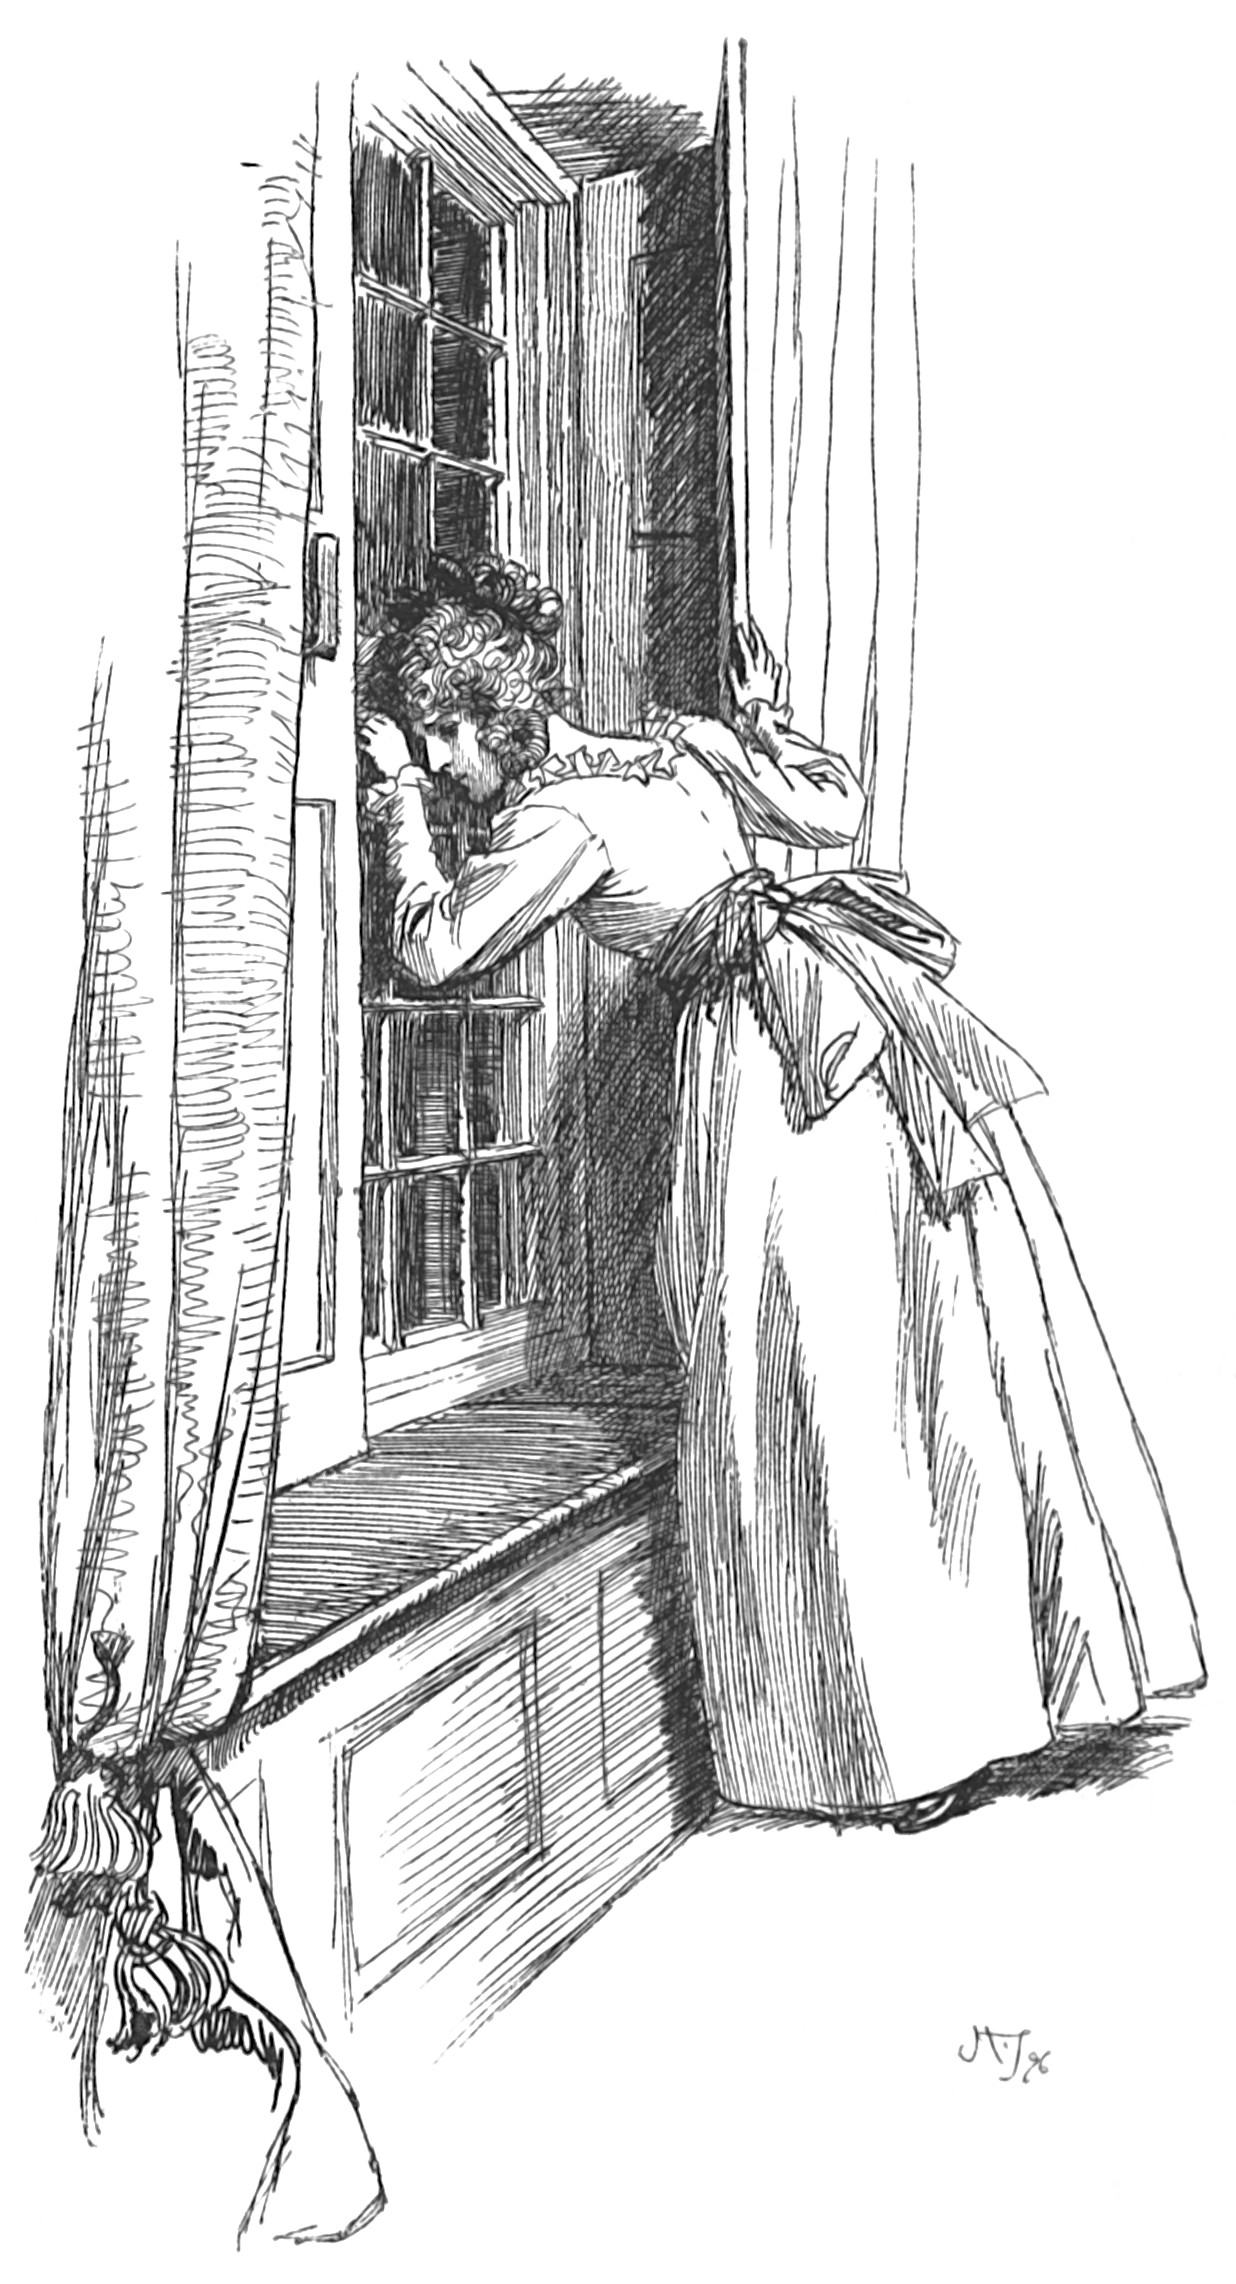
\includegraphics[width=.8\linewidth]{43shutter}
		\caption{Opened a window shutter}
	\end{figure}
\end{a4}

\begin{letter}
	\begin{figure}[tbph]
		\centering
		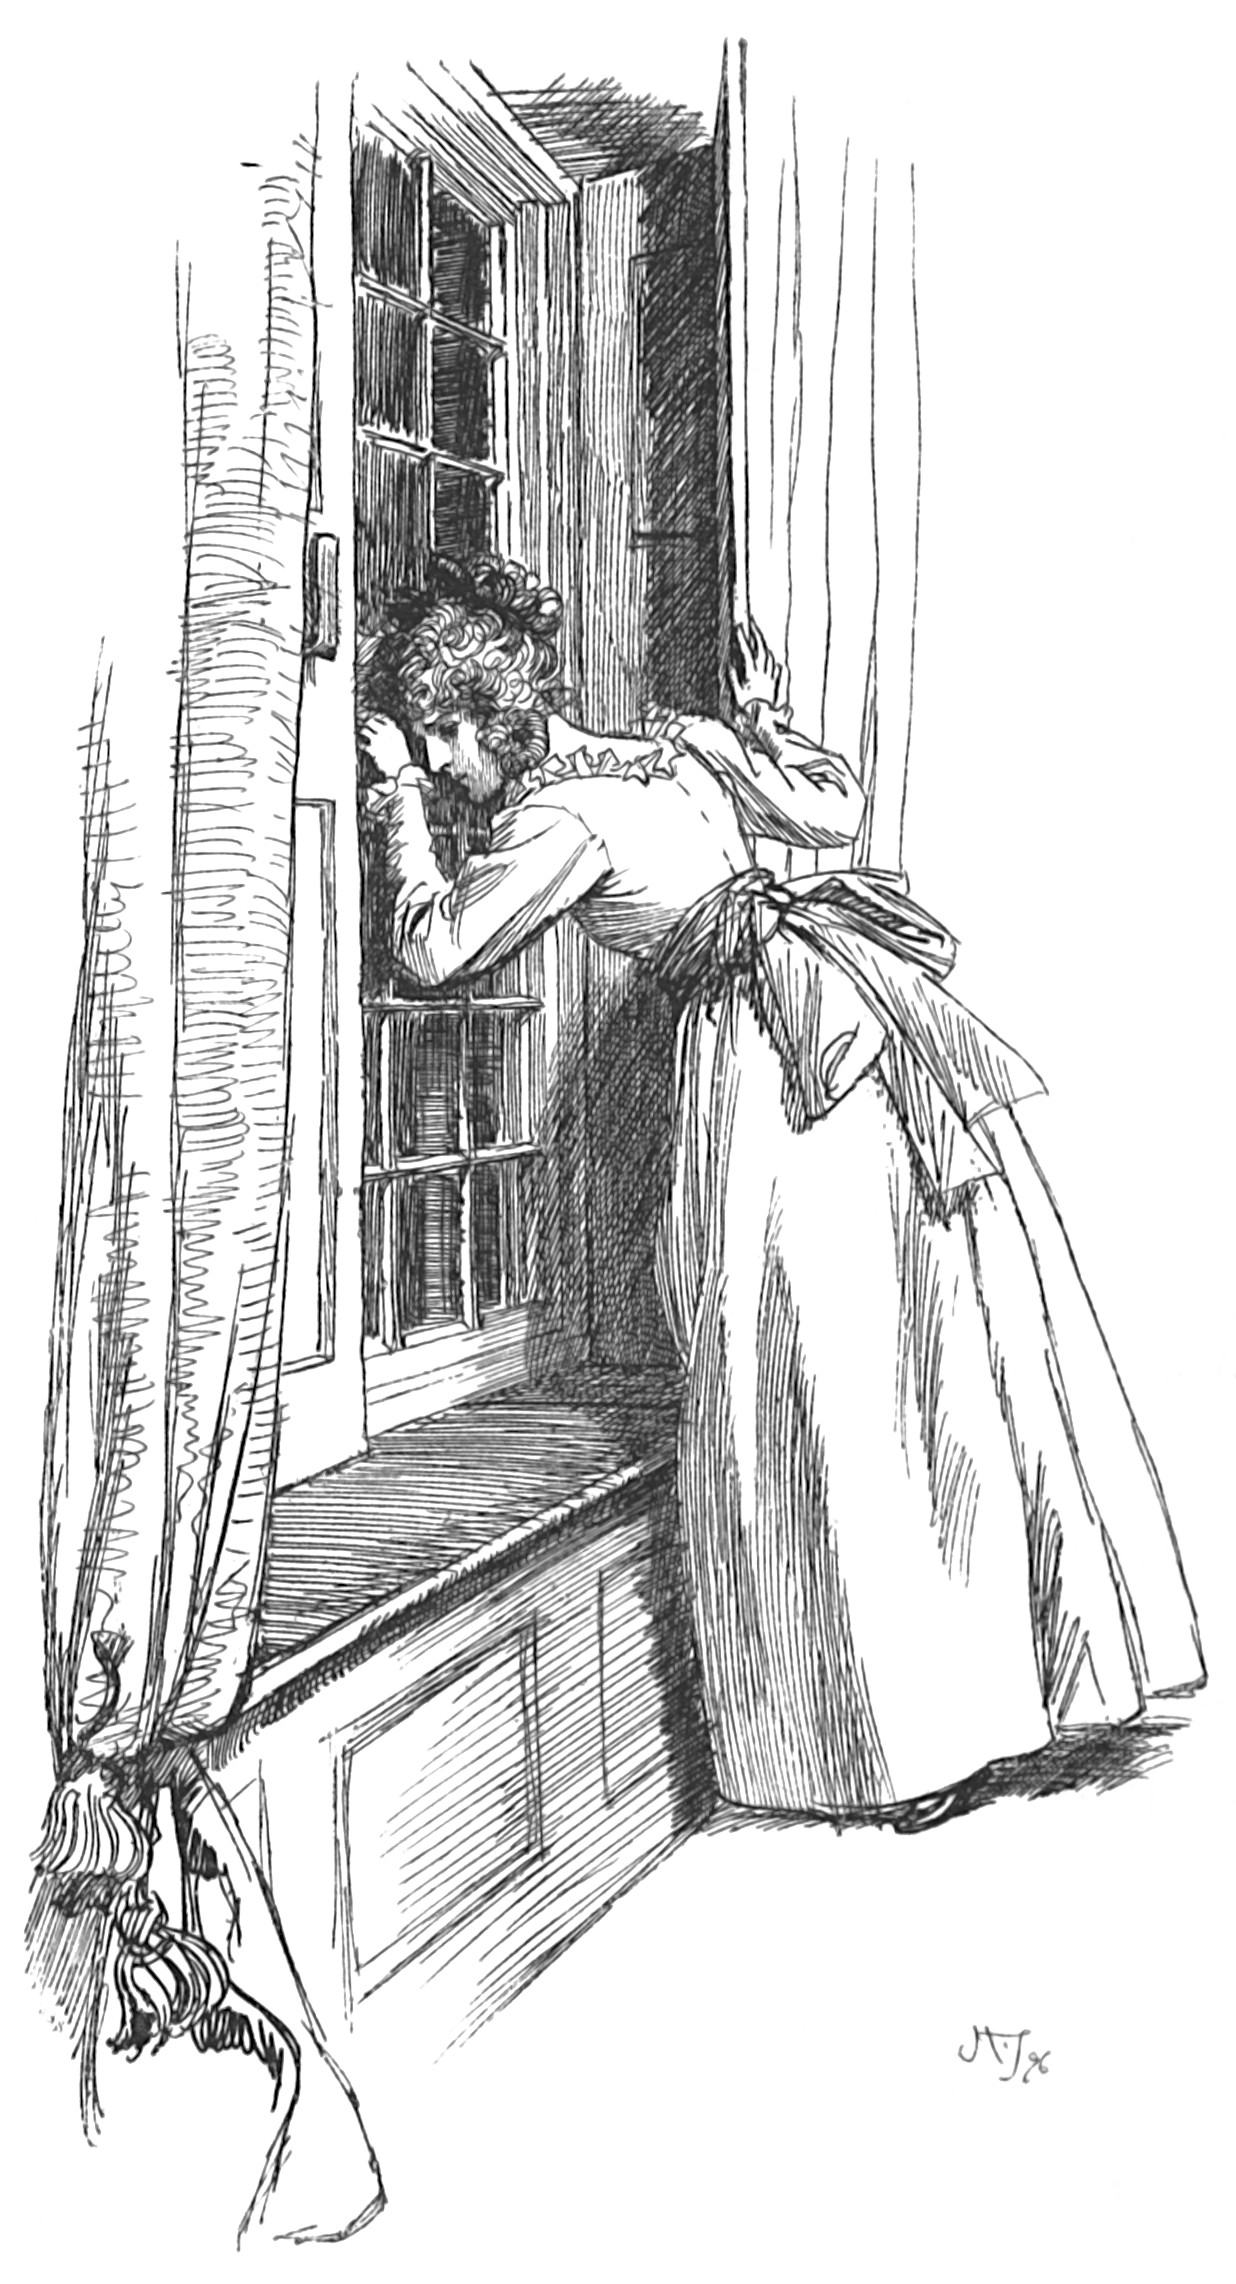
\includegraphics[width=.9\linewidth]{43shutter}
		\caption{Opened a window shutter}
	\end{figure}
\end{letter}

Never in her life had Elinor found it so difficult to be calm, as at that moment. The knowledge of what her mother must be feeling as the carriage stopt at the door—of her doubt—her dread—perhaps her despair!—and of what \textit{she} had to tell!—with such knowledge it was impossible to be calm. All that remained to be done was to be speedy; and, therefore staying only till she could leave Mrs Jennings's maid with her sister, she hurried down stairs.

The bustle in the vestibule, as she passed along an inner lobby, assured her that they were already in the house. She rushed to the drawing-room,—she entered it,—and saw only Willoughby.